\documentclass[11pt,a4paper]{book}
\usepackage[T1]{fontenc}
\usepackage{isabelle,isabellesym}
\usepackage{latexsym}
\usepackage{graphicx}
\usepackage{pdfsetup}
\usepackage[english]{babel}
\usepackage{ifthen}

\urlstyle{rm}
\isabellestyle{it}

\pagestyle{myheadings}

\addtolength{\hoffset}{-1,5cm}
\addtolength{\textwidth}{4cm}
\addtolength{\voffset}{-2cm}
\addtolength{\textheight}{4cm}

%subsection instead of section to make the toc readable
\renewcommand{\thesubsection}{\arabic{subsection}}
\renewcommand{\setisabellecontext}[1]{\markright{Theory~#1}}

%remove spaces from the isabelle environment (trivlist makes them too large)
\renewenvironment{isabelle}
{\begin{isabellebody}}
{\end{isabellebody}}

\renewcommand{\isacommand}[1]{\ifthenelse{\equal{#1}{lemma}}
{\par\isakeyword{#1}}{\isakeyword{#1}}}

\begin{document}

\title{Java Source and Bytecode Formalizations in Isabelle: Bali}
\author{Gerwin Klein \and Tobias Nipkow \and David von Oheimb \and
  Leonor Prensa Nieto \and Norbert Schirmer \and Martin Strecker}
\maketitle

\tableofcontents

\begin{center}
  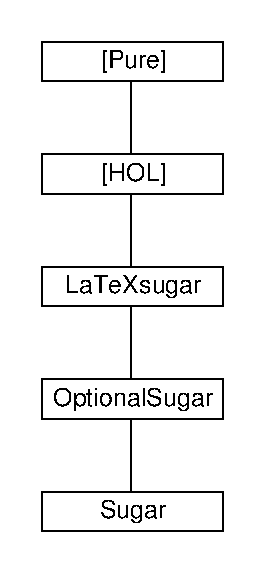
\includegraphics[scale=0.7]{session_graph}
\end{center}

\parindent 0pt\parskip 0.5ex
\chapter{Overview}
These theories, called Bali,  model and analyse different aspects of the 
JavaCard \textbf{source language}. 
The basis is an abstract model of the JavaCard source language. 
On it, a type system, an operational semantics and an axiomatic semantics 
(Hoare logic) are built. The execution of a wellformed program (with respect to
the type system) according to the operational semantics is proved to be 
typesafe. The axiomatic semantics is proved to be sound and relative complete 
with respect to the operational semantics.

We have modelled large parts of the original JavaCard source language. It models
features such as:
\begin{itemize}
\item The basic ``primitive types'' of Java 
\item Classes and related concepts 
\item Class fields and methods
\item Instance fields and methods
\item Interfaces and related concepts 
\item Arrays
\item Static initialisation
\item Static overloading of fields and methods
\item Inheritance, overriding and hiding of methods, dynamic binding
\item All cases of abrupt termination
      \begin{itemize}
        \item Exception throwing and handling
        \item \texttt{break}, \texttt{continue} and \texttt{return} 
      \end{itemize}
\item Packages
\item Access Modifiers (\texttt{private}, \texttt{protected}, \texttt{public})
\item A ``definite assignment'' check
\end{itemize}

The following features are missing in Bali wrt.{} JavaCard:
\begin{itemize}
\item Some primitive types (\texttt{byte, short})
\item Syntactic variants of statements
  (\texttt{do}-loop, \texttt{for}-loop)
\item Interface fields
\item Inner Classes
\end{itemize}

In addition, features are missing that are not part of the JavaCard
language, such as multithreading and garbage collection. No attempt
has been made to model peculiarities of JavaCard such as the applet
firewall or the transaction mechanism.


Overview of the theories:
\begin{description}
\item[Basis] 
Some basic definitions and settings not specific to JavaCard but missing in HOL.

\item[Table]
Definition and some properties of a lookup table to map various names 
(like class names or method names) to some content (like classes or methods).

\item[Name]
Definition of various names (class names, variable names, package names,...)

\item[Value]
JavaCard expression values (Boolean, Integer, Addresses,...)

\item[Type]
JavaCard types. Primitive types (Boolean, Integer,...) and reference types 
(Classes, Interfaces, Arrays,...)

\item[Term]
JavaCard terms. Variables, expressions and statements.

\item[Decl]
Class, interface and program declarations. Recursion operators for the
class and the interface hierarchy. 

\item[TypeRel]
Various relations on types like the subclass-, subinterface-, widening-, 
narrowing- and casting-relation.

\item[DeclConcepts]
Advanced concepts on the class and interface hierarchy like inheritance, 
overriding, hiding, accessibility of types and members according to the access 
modifiers, method lookup.

\item[WellType]
Typesystem on the JavaCard term level.

\item[DefiniteAssignment]
The definite assignment analysis on the JavaCard term level.

\item[WellForm]
Typesystem on the JavaCard class, interface and program level.

\item[State]
The program state (like object store) for the execution of JavaCard.
Abrupt completion (exceptions, break, continue, return) is modelled as flag
inside the state.

\item[Eval]
Operational (big step) semantics for JavaCard.

\item[Example]
An concrete example of a JavaCard program to validate the typesystem and the
operational semantics.

\item[Conform]
Conformance predicate for states. When does an execution state conform to the
static types of the program given by the typesystem.

\item[DefiniteAssignmentCorrect]
Correctness of the definite assignment analysis. If the analysis regards a variable as definitely assigned at a
certain program point, the variable will actually be assigned there during execution.

\item[TypeSafe]
Typesafety proof of the execution of JavaCard. ''Welltyped programs don't go
wrong'' or more technical: The execution of a welltyped JavaCard program 
preserves the conformance of execution states.

\item[Evaln]
Copy of the operational semantics given in theory Eval expanded with an annotation
for the maximal recursive depth. The semantics is not altered. The annotation
is needed for the soundness proof of the axiomatic semantics.

\item[Trans]
A smallstep operational semantics for JavaCard.

\item[AxSem]
An axiomatic semantics (Hoare logic) for JavaCard.

\item[AxSound]
The soundness proof of the axiomatic semantics with respect to the operational
semantics.

\item[AxCompl]
The proof of (relative) completeness of the axiomatic semantics with respect
to the operational semantics. 

\item[AxExample]
An concrete example of the axiomatic semantics at work, applied to prove 
some properties of the JavaCard example given in theory Example.
\end{description}


\chapter{Basis}
\input{Basis}

\chapter{Table}
\input{Table}    

\chapter{Name}
\input{Name}

\chapter{Value}     
\input{Value}

\chapter{Type}
\input{Type}      

\chapter{Term}
\input{Term}     

\chapter{Decl}
\input{Decl}          

\chapter{TypeRel}
\input{TypeRel}   

\chapter{DeclConcepts}
\input{DeclConcepts}  

\chapter{WellType}
\input{WellType}

\chapter{DefiniteAssignment}
\input{DefiniteAssignment}

\chapter{WellForm}
\input{WellForm}

\chapter{State}
\input{State}    

\chapter{Eval}
\input{Eval}          

\chapter{Example}
\input{Example}  

\chapter{Conform}
\input{Conform}       

\chapter{DefiniteAssignmentCorrect}
\input{DefiniteAssignmentCorrect}

\chapter{TypeSafe}
\input{TypeSafe}

\chapter{Evaln}
\input{Evaln}         

\chapter{Trans}
\input{Trans}         

\chapter{AxSem}
\input{AxSem}      

\chapter{AxSound}
\input{AxSound}    

\chapter{AxCompl}
\input{AxCompl}    

\chapter{AxExample}
\input{AxExample}  

%\bibliographystyle{abbrv}
%\bibliography{root}

\end{document}
